% Vorlage fuer latex-beamer-Praesentationen unter Verwendung des Corporate 
% Designs der Uni.
%
% Basiert auf der alten Vorlage von Carsten Bockelmann 
% (bockelmann@ant.uni-bremen.de), angepasst an das Corporate Design von 
% Henning Paul (paul@ant.uni-bremen.de) unter Verwendung der Vorlage von
% Dirk Lorenz und Kristan Bredies aus dem Zentrum fuer Technomathematik
% ({dlorenz,kbredies}@math.uni-bremen.de)

\documentclass[10pt]{beamer}

\mode<presentation>
{
  % Das ANT-Theme benutzen
  % Titel in Kopfzeile, kleine Navigationselemente, Seitennummer anzeigen,
  % Autor dauerhaft eingeblendet lassen
  % \usetheme[headlinetitle,navline=small,footlinenumber,footlineauthor]{ANT}

  % Autor nicht dauerhaft einblenden
   \usetheme[headlinetitle,navline=small,footlinenumber]{Bremen}

  %
  % Die vollstaendige Dokumentation zu unserem Theme findet sich in der Datei 
  % beamerZeTeMdoc.pdf, da es auf dem Theme der Technomathematiker aus dem 
  % ZeTeM basiert.
  %
  % Es koennen bis zu zwei zusaetzliche Logos (zu unserer Ameise oben links
  % und dem Uni-Logo unten links) hinzugefuegt werden, diese erscheinen dann
  % rechts neben dem Uni-Logo.
  % \partnerlogo{
	% \includegraphics[height=2.6\baselineskip]{TZI.pdf}}
  % \secondarypartnerlogo{
	% \includegraphics[height=2.6\baselineskip]{DFG_zweizeilig_blau.pdf}}

  % Dieses sind Standard-latex-beamer-Optionen:
  %
  % Der mathematische Schriftsatz ist mit Serifen
  \usefonttheme[onlymath]{serif}
  % Noch nicht aufgedeckte Punkte erscheinen ausgegraut
  \setbeamercovered{transparent}
  % Bild-/Tabellenueberschriften sind sehr klein
  \setbeamerfont{caption}{size=\tiny}

}


%\usepackage[german]{babel}
% oder was auch immer

\usepackage[utf8]{inputenc}
% oder was auch immer


\usepackage{hyperref}
\hypersetup{
    pdftitle={},
    pdfsubject={},
    pdfauthor={Max Mustermann},
    pdfkeywords={},
    % pdfpagemode=None, %deprecated
    plainpages=false,
    pdfstartview=Fit,
    breaklinks=true,
    colorlinks=false,
    pdfhighlight=/N,
    % define colors, even if not used
    linkcolor=blue,
    citecolor=blue,
    urlcolor=blue,
    citebordercolor=1 1 1,
    filebordercolor=1 1 1,
    linkbordercolor=1 1 1,
    menubordercolor=1 1 1,
    % pagebordercolor=1 1 1, %deprecated
    urlbordercolor=1 1 1,
    % pdfborder=1 1 1 %erzeugt fehler im footer
  }

\title{Property Oriented Testing}
\author{Sadik Özoguz}
\institute{Universit{\"a}t Bremen}
\date[02.02.2018]{2. Februar 2018}

\newcommand{\W}{\mathcal{W}}
\newcommand{\F}{\mathcal{F}}

\subject{Presentation}
\AtBeginSection[]
{
  \begin{frame}
    \frametitle{Überblick}
    \tableofcontents[currentsection]
  \end{frame}
}

% Hier beginnt der redaktionelle Inhalt


\begin{document}

\begin{frame}
  \titlepage
\end{frame}

\section*{Überblick}
\begin{frame}<beamer>
  \frametitle{Überblick}
  \tableofcontents
\end{frame}

\section{Einleitung / Motivation}

\begin{frame}
  \frametitle{Motivation}
  \begin{itemize}
    \item MBT: Modell $\rightarrow$ (vollständige) Test Suite
    \item Je größer die Test Suite, desto teurer das Testen
    \item<2-> Stattdessen: Nachweis einer Eigenschaft
    \item<3-> Ziel: Kleinere Testsuite, aber vollständig bezüglich dieser Eigenschaft
  \end{itemize}
\end{frame}

\section{DFSM}
\subsection{Definition}
\begin{frame}
  \frametitle{DFSM}

  \begin{definition}[Deterministische Finite State Machine]
    Eine deterministische Finite State Machine (DFSM) ist ein 5-Tupel $$M=(Q,q_0,\Sigma_I,\Sigma_O,h)$$
    $Q$: Zustandsraum\\
    $\Sigma_I$, $\Sigma_O$ : Ein-, Ausgabealphabet\\
    $h \subseteq Q \times \Sigma_I \times \Sigma_O \times Q$ : Übergangsrelation 
  \end{definition}
  Deterministisch: $(q,x,y_1,q_1),(q,x,y_2,q_2) \in h: (y_1 = y_2 \wedge q_1 = q_2)$
\end{frame}

\subsection{Eigenschaften}
\begin{frame}
\frametitle{FSM Eigenschaften}
\begin{itemize}
  \item<1-> Vollständig (\emph{input complete})$$\forall q\in Q, x\in \Sigma_I : \exists y \in \Sigma_O, q'\in Q : (q,x,y,q')\in h$$
  \item<2-> Die Sprache eines Zustandes $q \in Q$ ist eine Menge von Eingabe-/Aus\-gabefolgen $$L(q)= \{\overline{x}/\overline{y}\ | \exists q' \in Q : (q,\overline{x}, \overline{y}, q') \in h \}$$
  \item<3-> I/O-äquivalent: $L(q_1) = L(q_2)$ bzw. $L(M_1) = L(M_2)$ $$q_1 \sim q_2, M_1 \sim M_2$$
  \item<4-> Minimal: Wenn keine zwei Zustände einer DFSM zueinander äquivalent sind, ist die DFSM \emph{minimal}.
\end{itemize}
\end{frame}

\begin{frame}
\frametitle{Beispiel: Garage Door Controller}

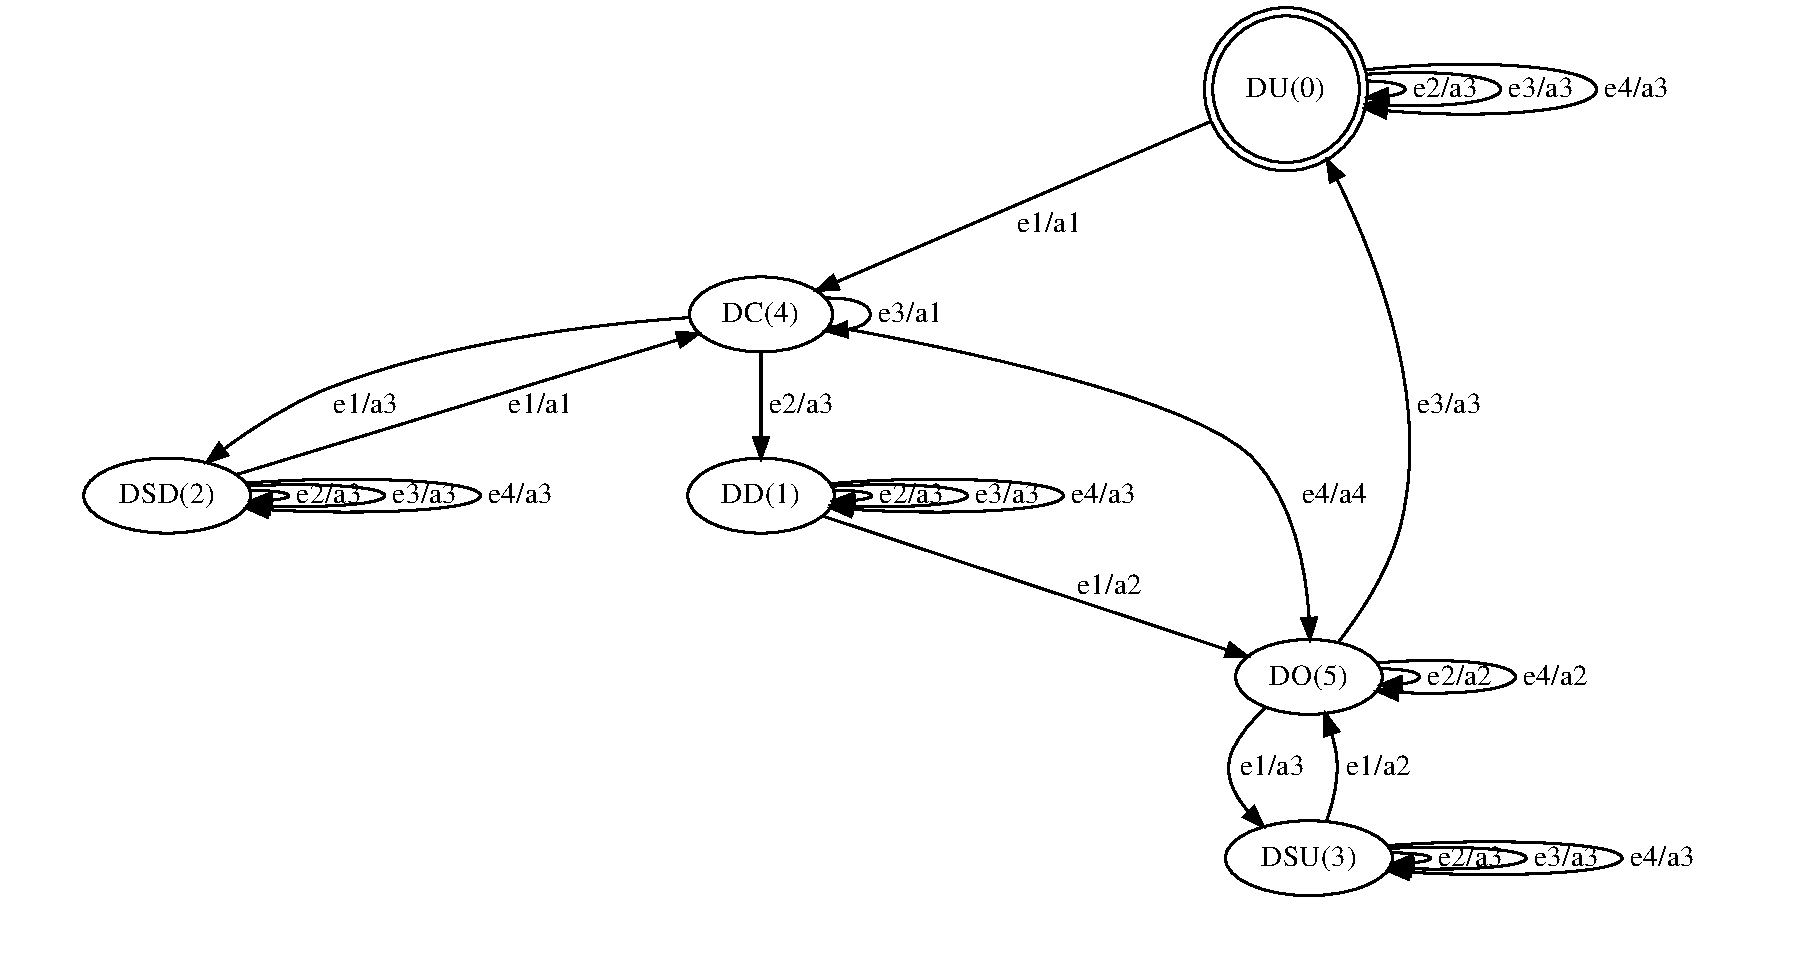
\includegraphics[width=\textwidth]{images/gdc}

\end{frame}


\begin{frame}
\frametitle{Beispiel: Garage Door Controller}
\begin{columns}[T] % align columns
\begin{column}{.48\textwidth}

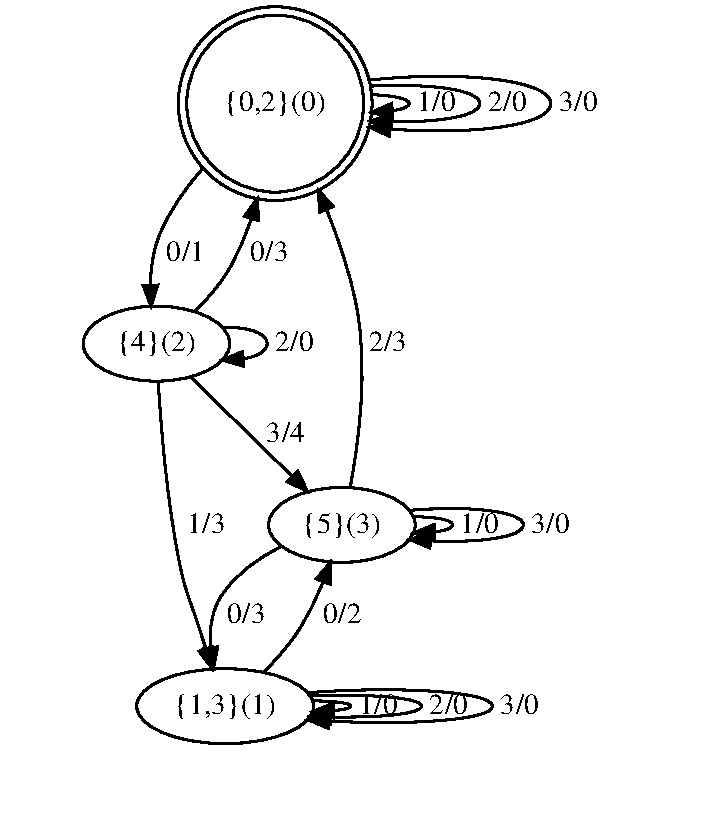
\includegraphics[width=\textwidth]{images/gdc_min}
\end{column}%
\hfill%
\begin{column}{.48\textwidth}
\begin{itemize}
  \item e1: Fernbedienung gedrückt
  \item e2: Sensor "Tür ist unten"
  \item e3: Sensor "Tür ist oben"
  \item e4: Sensor "Lichtschrank aktiviert"
\end{itemize}
\end{column}%
\end{columns}
\end{frame}

\section{Conformance Testing}
\subsection{$\W$-Methode}
\begin{frame}
  \frametitle{$\W$-Methode}
  \begin{definition}[$\W$-Methode]
  Gegeben ist eine vollständige, minimale DFSM $M$ mit $n$ Zuständen, dann definiert die $\W$-Methode eine vollständige Testsuite T für $M$ mit
  $$T_\W(M) = V.\bigcup\limits_{i=0}^{m-n+1}\Sigma_I^i.W$$
  bzgl. der Fault Model $\F(M, \sim, \texttt{Dom})$.
  \end{definition}
  \pause
  \begin{itemize}
    \item<2-> $V$ : State Cover
    \item<3-> $W$ : Characterization Set
    \item<4-> $m \in \mathbb{N}$ mit $m \geq n$ (max. Zustände in der Implementierung)
    \item<5-> $\texttt{Dom} = DFSM_C(\Sigma_I, \Sigma_O, m)$ 
  \end{itemize}

\end{frame}

\subsection{$H$-Methode}
\begin{frame}
  \frametitle{$H$-Methode}

\end{frame}

\subsection[Subsection 1]{First Subsection in First Section}

\begin{frame}
  \frametitle{What Are Prime Numbers?}
  \begin{definition}
  A \alert{prime number} is a number that has exactly two divisors.
  \end{definition}
\end{frame}

\end{document}


